\problemname{AVL++}

\illustration{0.25}{plus.jpg}{Image by \href{https://www.shutterstock.com/g/Ilya+Glukhov}{Ilya Klukhov (Shutterstock)}, Used under license}

An AVL tree, named after its inventors, Adelson-Velskii and Landis, is a binary search tree
with an additional constraint that keeps the tree balanced. The \emph{balance factor} of
a node $x$, denoted $\mathit{bf}(x)$, is defined to be $H(x_R) - H(x_L)$, where $H(\,)$
denotes height, $x_R$ is the right subtree of $x$, and $x_L$ is the left subtree of $x$.
(The height of a (sub)tree is the number of edges in the longest simple path from its root
to any leaf. It follows that the height of a tree containing a single node is $0$.
The height of the empty tree, i.e., the tree with no nodes, is typically defined to be $-1$.)
In an AVL tree, the only balance factors permitted are $\{-1,0,1\}$, i.e., $|\mathit{bf}(x)| \leq 1$
for every node $x$.

Two AVL trees $T_1$ and $T_2$ are \emph{isomorphic} if there is a bijection
$f : X_1 \rightarrow X_2$, where $X_1$ is the set of nodes in $T_1$, and $X_2$ is the set
of nodes in $T_2$, such that for all $x,y \in X_1$, $y$ is the right (respectively, left) child
of $x$ in $T_1$ if and only if $f(y)$ is the right (respectively, left) child of $f(x)$ in $T_2$.
In other words, two AVL trees are isomorphic if they have the same ``shape''
(we are not concerned with the values stored in the nodes).

Now consider one way to generalize the AVL constraint. Let $m \geq 0$ be an integer, and
define an \mbox{AVL-$m$} tree to be a binary search tree satisfying $|\mathit{bf}(x)| \leq m$
for every node $x$. This gives rise to an interesting question: How many differently shaped
(non-isomorphic) \mbox{AVL-$m$} trees are there with a given height $h$? The figure below
illustrates the answer when $m=2$ and $h=2$.

\begin{figure}[!h]
\centering
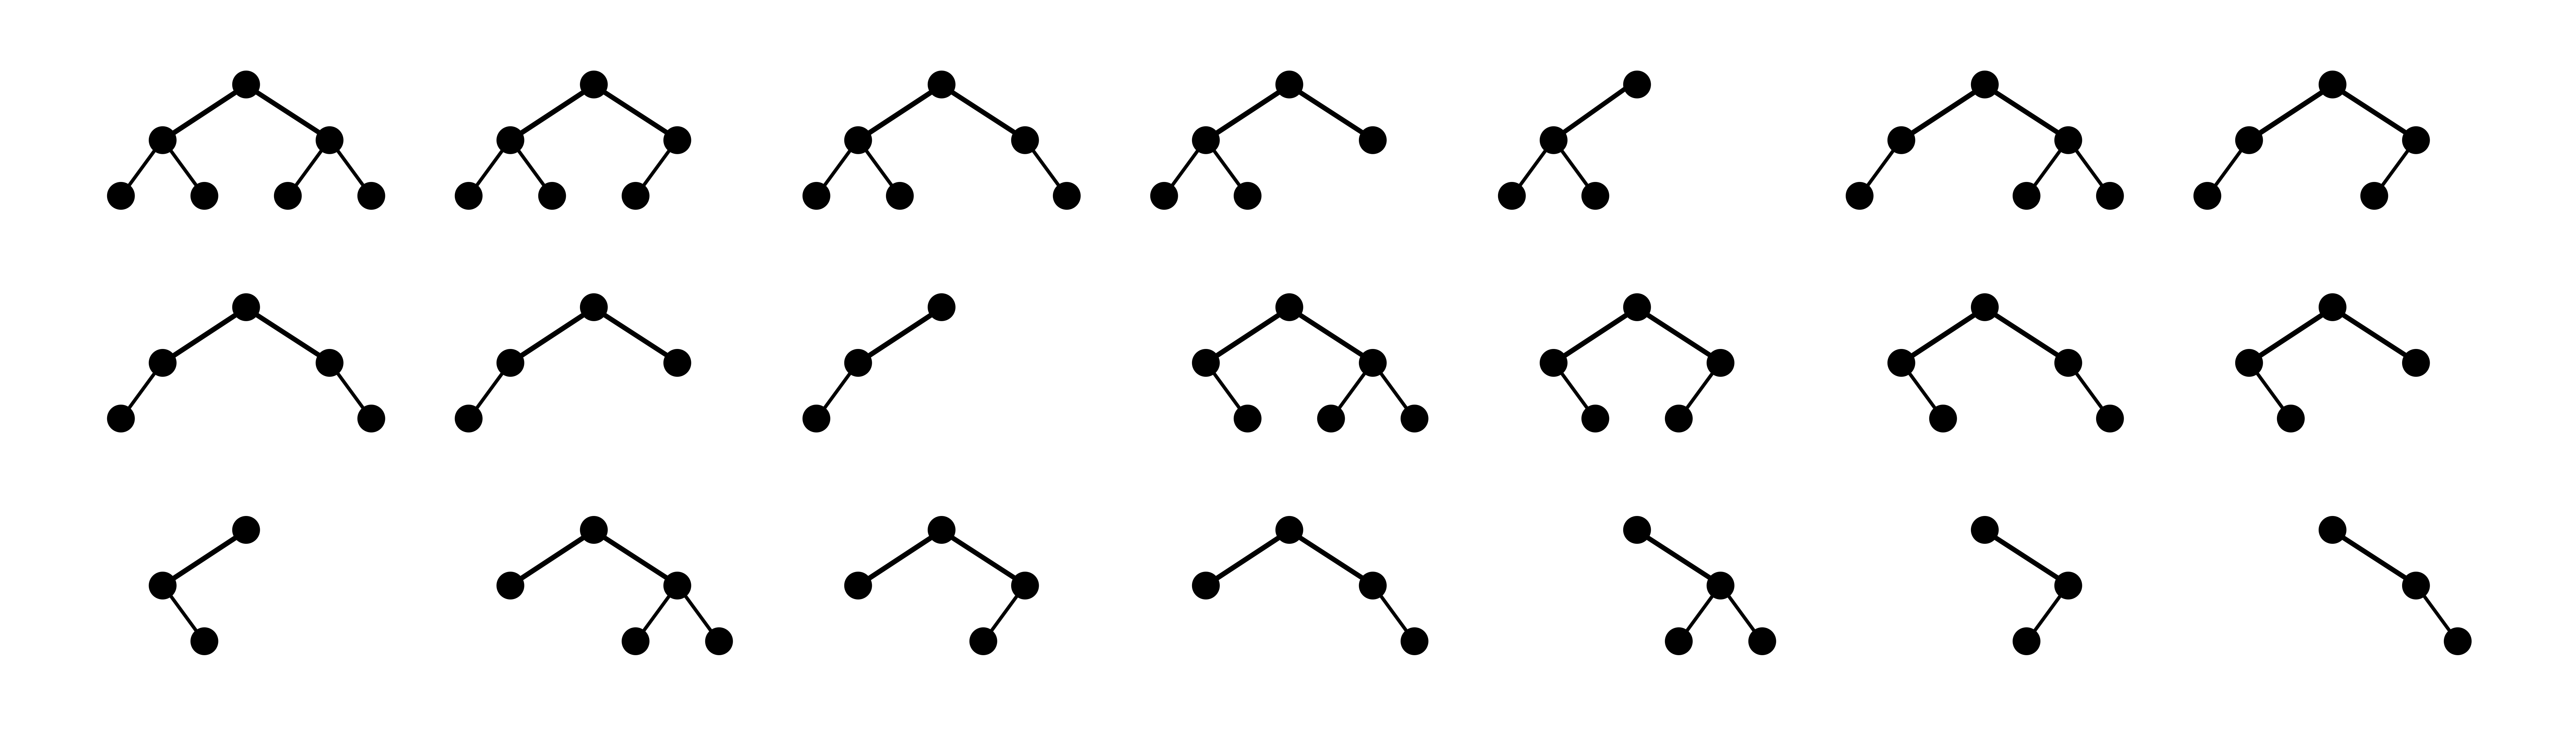
\includegraphics[width=0.75\textwidth]{trees.png}
\caption{There are $21$ \mbox{AVL-$2$} trees with height $2$}
\end{figure}


\section*{Input}

The first line of input contains an integer $Q$ $(1 \leq Q \leq 100)$ indicating the number
of queries to follow.  Each of the next $Q$ lines contains a query consisting of two
space-separated integers $m$ and $h$ $(0 \leq m \leq 100, 0 \leq h \leq 1000)$.


\section*{Output}

For each query, output a line containing the number of non-isomorphic \mbox{AVL-$m$} trees
with height $h$. Since these numbers may be large, report each answer mod $(10^9+7)$.

